% Generated by AP Math GOLD PILOT deterministic Python generator.
% input id: 01_coordinate_perpendicular
\documentclass{article}
\usepackage[margin=1cm]{geometry}
\def\pgfsysdriver{pgfsys-dvisvgm.def}
\usepackage{fontspec}
\setmainfont{Malgun Gothic}
\setsansfont{Malgun Gothic}
\usepackage{amsmath}
\usepackage{amssymb}
\usepackage{pgfplots}
\pgfplotsset{compat=1.18}
\pagestyle{empty}
\begin{document}
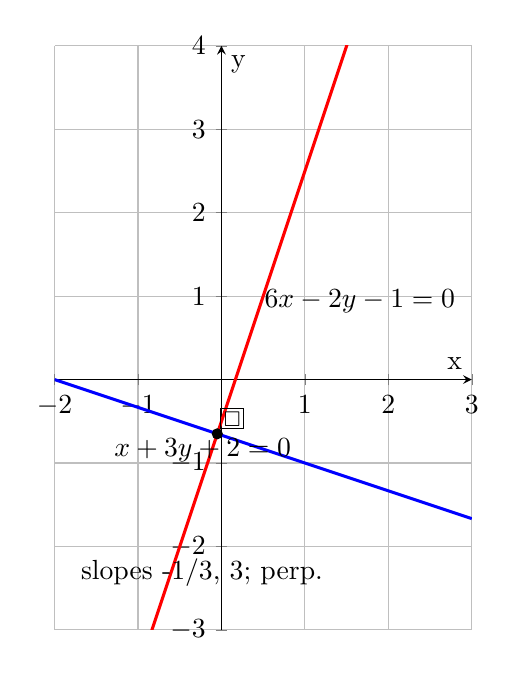
\begin{tikzpicture}
\begin{axis}[width=13cm,height=9cm,axis equal image,axis lines=middle,grid=major,xmin=-2,xmax=3,ymin=-3,ymax=4,xlabel={x},ylabel={y},clip=true]
\addplot[blue, solid, line width=1.1pt] coordinates {(-2,0) (-1.9375,-0.020833) (-1.875,-0.041667) (-1.8125,-0.0625) (-1.75,-0.083333) (-1.6875,-0.104167) (-1.625,-0.125) (-1.5625,-0.145833) (-1.5,-0.166667) (-1.4375,-0.1875) (-1.375,-0.208333) (-1.3125,-0.229167) (-1.25,-0.25) (-1.1875,-0.270833) (-1.125,-0.291667) (-1.0625,-0.3125) (-1,-0.333333) (-0.9375,-0.354167) (-0.875,-0.375) (-0.8125,-0.395833) (-0.75,-0.416667) (-0.6875,-0.4375) (-0.625,-0.458333) (-0.5625,-0.479167) (-0.5,-0.5) (-0.4375,-0.520833) (-0.375,-0.541667) (-0.3125,-0.5625) (-0.25,-0.583333) (-0.1875,-0.604167) (-0.125,-0.625) (-0.0625,-0.645833) (0,-0.666667) (0.0625,-0.6875) (0.125,-0.708333) (0.1875,-0.729167) (0.25,-0.75) (0.3125,-0.770833) (0.375,-0.791667) (0.4375,-0.8125) (0.5,-0.833333) (0.5625,-0.854167) (0.625,-0.875) (0.6875,-0.895833) (0.75,-0.916667) (0.8125,-0.9375) (0.875,-0.958333) (0.9375,-0.979167) (1,-1) (1.0625,-1.020833) (1.125,-1.041667) (1.1875,-1.0625) (1.25,-1.083333) (1.3125,-1.104167) (1.375,-1.125) (1.4375,-1.145833) (1.5,-1.166667) (1.5625,-1.1875) (1.625,-1.208333) (1.6875,-1.229167) (1.75,-1.25) (1.8125,-1.270833) (1.875,-1.291667) (1.9375,-1.3125) (2,-1.333333) (2.0625,-1.354167) (2.125,-1.375) (2.1875,-1.395833) (2.25,-1.416667) (2.3125,-1.4375) (2.375,-1.458333) (2.4375,-1.479167) (2.5,-1.5) (2.5625,-1.520833) (2.625,-1.541667) (2.6875,-1.5625) (2.75,-1.583333) (2.8125,-1.604167) (2.875,-1.625) (2.9375,-1.645833) (3,-1.666667)};
\addplot[red, solid, line width=1.1pt] coordinates {(-2,-6.5) (-1.9375,-6.3125) (-1.875,-6.125) (-1.8125,-5.9375) (-1.75,-5.75) (-1.6875,-5.5625) (-1.625,-5.375) (-1.5625,-5.1875) (-1.5,-5) (-1.4375,-4.8125) (-1.375,-4.625) (-1.3125,-4.4375) (-1.25,-4.25) (-1.1875,-4.0625) (-1.125,-3.875) (-1.0625,-3.6875) (-1,-3.5) (-0.9375,-3.3125) (-0.875,-3.125) (-0.8125,-2.9375) (-0.75,-2.75) (-0.6875,-2.5625) (-0.625,-2.375) (-0.5625,-2.1875) (-0.5,-2) (-0.4375,-1.8125) (-0.375,-1.625) (-0.3125,-1.4375) (-0.25,-1.25) (-0.1875,-1.0625) (-0.125,-0.875) (-0.0625,-0.6875) (0,-0.5) (0.0625,-0.3125) (0.125,-0.125) (0.1875,0.0625) (0.25,0.25) (0.3125,0.4375) (0.375,0.625) (0.4375,0.8125) (0.5,1) (0.5625,1.1875) (0.625,1.375) (0.6875,1.5625) (0.75,1.75) (0.8125,1.9375) (0.875,2.125) (0.9375,2.3125) (1,2.5) (1.0625,2.6875) (1.125,2.875) (1.1875,3.0625) (1.25,3.25) (1.3125,3.4375) (1.375,3.625) (1.4375,3.8125) (1.5,4) (1.5625,4.1875) (1.625,4.375) (1.6875,4.5625) (1.75,4.75) (1.8125,4.9375) (1.875,5.125) (1.9375,5.3125) (2,5.5) (2.0625,5.6875) (2.125,5.875) (2.1875,6.0625) (2.25,6.25) (2.3125,6.4375) (2.375,6.625) (2.4375,6.8125) (2.5,7) (2.5625,7.1875) (2.625,7.375) (2.6875,7.5625) (2.75,7.75) (2.8125,7.9375) (2.875,8.125) (2.9375,8.3125) (3,8.5)};
\addplot[only marks,mark=*,mark size=1.8pt,black] coordinates {(-0.05,-0.65)};
\node[anchor=south west] at (axis cs:-1.4,-1.1) {$x+3y+2=0$};
\node[anchor=north west] at (axis cs:0.4,1.2) {$6x-2y-1=0$};
\node[anchor=south west] at (axis cs:-1.8,-2.6) {slopes -1/3, 3; perp.};
\node[draw,inner sep=1pt,font=\scriptsize] at (axis cs:0.13,-0.47) {$\square$};
\end{axis}
\end{tikzpicture}
\end{document}
